

\chapter{Spare Parts} \hypertarget{def:spare}{}

The PICSimLab has a window that allows the connection of spare parts to the microcontroller, it can be accessed through the menu `` Modules-> Spare parts ''.

The main window has the menu with the following functions:
\begin{itemize}
 \item File
 \begin{itemize}
 \item New configuration - Clear the spare parts window 
 \item Save configuration - Saves the current settings of the spare parts into .pcf file
 \item Load configuration - Loads the settings from .pcf file
 \item Save pin alias - Saves the current pin alias to .ppa text file
 \item Load pin alias - Loads the pin alias from .ppa file
\end{itemize}
 \item Edit
 \begin{itemize}
 \item Clear pin alias - Clear the pin alias 
 \item Toggle pin alias - Enable/Disable pin alias use
 \item Edit pin alias - Open current pin alias .ppa file in text editor
 \item Reload pin alias - Reload the current .ppa pin alias file (need after edit .ppa file) 
 \item Zoom in - Increase draw scale
 \item Zoom out - Decrease draw scale
\end{itemize}
 \item Inputs
 \begin{itemize}
  \item DS1621 (Temperature I2C) -  Adds a I2C temperature sensor 
  \item Encoder - Adds a rotary quadrature encoder with push button
  \item FM50 (Temperature) - Adds a analog temperature sensor
  \item Fixed Voltage -  Adds a analog fixed voltage reference
  \item Gamepad - Adds a gamepad
  \item Gamepad (Analogic) - Adds a gamepad with one analogic output 
  \item Keypad -  Adds one matrix keypad
  \item LDR - Adds a light dependent resistor 
  \item LM35 (Temperature) - Adds a analog temperature sensor
  \item MPU6050 - Adds a accelerometer and gyroscope (only raw values)
  \item Potentiometers - Adds 4 potentiometers
  \item Potentiometers (Rotary) - Adds 4 rotary potentiometers
  \item Push Buttons - Adds 8 push buttons
  \item Push Buttons (Analogic) - Adds 8 push buttons with analog output
  \item SHT3X - Adds a analog temperature and humidity sensor
  \item Switches - Adds eight switches
  \item Ultrasonic HC-SR04 - Adds a ultrasonic range sensor
\end{itemize}
 \item{Outputs}
  \begin{itemize}
   \item 7 Segments Display -  Adds four multiplexed (or single) 7 segments displays
   \item 7 Segments Display (w/dec) -  Adds four multiplexed 7 segments displays with decoder
   \item Buzzer - Adds a active/passive buzzer
   \item DC Motor - Adds a DC motor with H-bridge and quadrature encoder 
   \item LCD hd44780 - Adds a text display hd44780
   \item LCD hd44780 I2C - Adds a text display hd44780 connect to one PCF8574 I2C converter
   \item LCD ili9340 - Adds a color graphic display ili9340 with touchscreen 
   \item LCD pcd8544 - Adds a monochrome graphic display pcd8544 (Nokia 5110)
   \item LCD pcf8833 - Adds a color graphic display pcf8833
   \item LCD ssd1306 - Adds a monochrome graphic display ssd1306
   \item LED Matrix - Adds a 8x8 LED matrix with MAX72xx controller 
   \item LEDs - Adds 8 red LEDs
   \item RGB LED - Adds one RGB LED 
   \item RGB LED WS2812B - Adds one or multiple addressable RGB LED 
   \item Servo Motor - Adds a servo motor
   \item Step Motor - Adds a step motor
 \end{itemize}
 \item{Others}
  \begin{itemize}
   \item ETH w5500 - Adds a ethernet shield w5500
   \item IO 74xx573 - Adds a 74xx573 octal latch
   \item IO 74xx595 - Adds a 74xx595 SIPO 8 bit shift register
   \item IO MCP23S17 - Adds a MCP23S17 serial SPI IO expander
   \item IO PCF8574 - Adds a PCF8574 serial I2C IO expander
   \item IO UART - Adds a UART serial port 
   \item Jumper Wires - Adds sixteen jumper wires 
   \item MEM 24CXXX - Adds a 24CXXX serial I2C EEPROM  memory
   \item RTC ds1307 - Adds a ds1307 real time clock 
   \item RTC pfc8563 - Adds a pfc8563 real time clock
   \item SD Card - Adds a SD card shield
   \item Temperature System - Adds a temperature control system
  \end{itemize}
\item{Virtual}
  \begin{itemize}
  \item D. Transfer Function - Adds a discrete transfer function mathematical model
  \item IO Virtual term - Adds a virtual serial terminal 
  \item Signal Generator - Adds a virtual signal generator
  \item Text Box - Adds a static text box
  \item VCD Dump - Adds a digital value file dump recorder 
  \item VCD Dump (Analogic) - Adds a analog value file dump recorder  
  \item VCD Play - Adds a digital value file dump player  
  \end{itemize}   
 \item Help
 \begin{itemize}
 \item Contents - Open Help window
 \item About - Show message about author and version
\end{itemize}
\end{itemize}


\begin{figure}[H]
\center
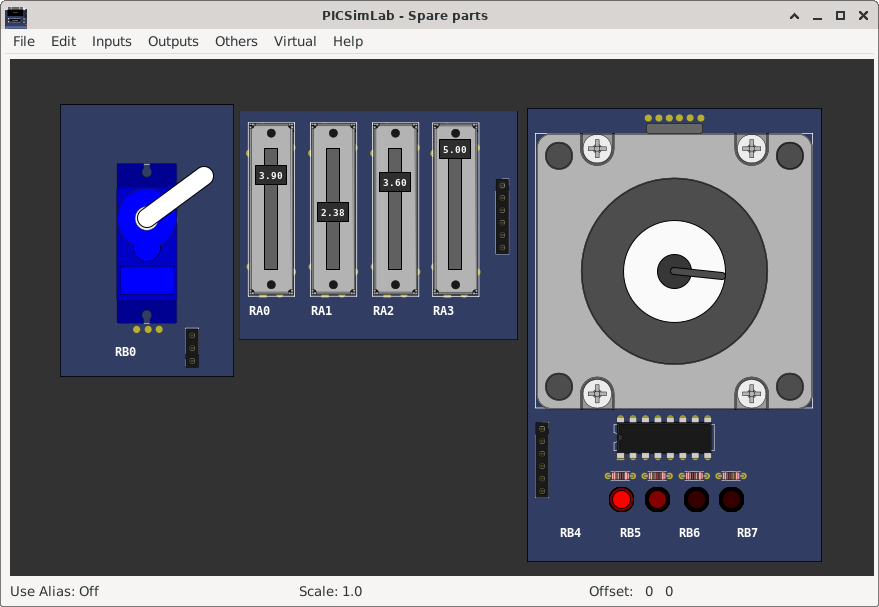
\includegraphics[width=0.99\textwidth]{img/spare.png} 
\end{figure} 

After adding the part, with a right click of the mouse you can access the options menu of the part with the options:
\begin{itemize}
 \item Properties - Opens the connection settings window
 \item Move - Unlocks the part to move
 \item Rotate - Change the orientation of part
 \item Delete - Remove part
 \item Help - Open Help window of part
 \item About - Show message about author and version of part
\end{itemize}


\begin{figure}[H]
\center
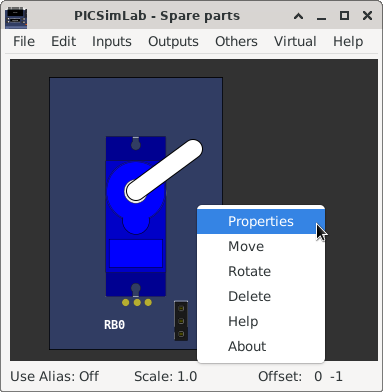
\includegraphics[width=0.60\textwidth]{img/spare_pmenu.png} 
\end{figure} 

\section{Pin Alias}

The pin alias support allows the user to place custom names on the pins making it easy to 
identify according to the project. 

When off the normal names are shown:
\begin{figure}[H]
\center
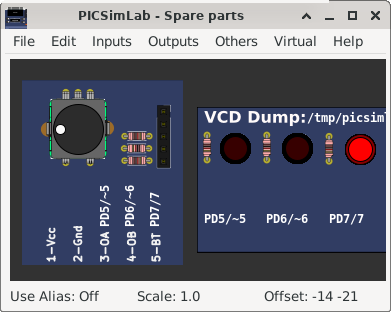
\includegraphics[width=0.80\textwidth]{img/pin_alias_off.png} 
\end{figure} 

When on the alias names are shown:
\begin{figure}[H]
\center
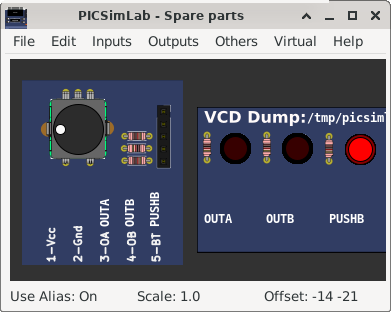
\includegraphics[width=0.80\textwidth]{img/pin_alias_on.png} 
\end{figure} 

To use:
\begin{enumerate}
 \item active the menu ``Edit->Clear pin alias'' to reset the pin alias file
 \item active the menu ``Edit->Edit pin alias'' to open pin alias file, change the names, save and close.
 \item active the menu ``Edit->Reload pin alias'' to load new alias
 \item active the menu ``Edit->Toggle pin alias'' to show new alias
\end{enumerate}


\section{Inputs}


\subsection{DS1621 (Temperature I2C)}


This part is DS1621 I2C temperature sensor. The measurement range is -55 to 125 °C.

\begin{figure}[H]
\center
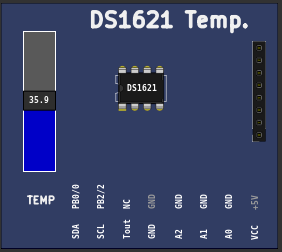
\includegraphics[width=0.5\textwidth]{img/part_ds1621.png} 
\end{figure} 


\href{https://lcgamboa.github.io/picsimlab_examples/parts_DS1621_(Temperature_I2C).html}{Examples}


\subsection{Encoder}

This part is a rotary quadrature encoder with push button. The output is twenty pulses per revolution.

\begin{figure}[H]
\center
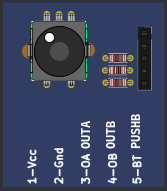
\includegraphics[width=0.25\textwidth]{img/part_encoder.png} 
\end{figure} 

\href{https://lcgamboa.github.io/picsimlab_examples/parts_Encoder.html}{Examples}
 
\subsection{FM50 (Temperature)}

This part is FM50 analog temperature sensor. The measurement range is -40 to 125 °C  and 
voltage output is 10mV/°C + 500mV.

\begin{figure}[H]
\center
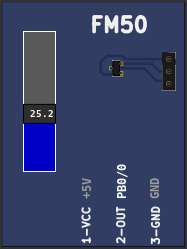
\includegraphics[width=0.3\textwidth]{img/part_fm50.png} 
\end{figure} 


\href{https://lcgamboa.github.io/picsimlab_examples/parts_FM50_(Temperature).html}{Examples}

\subsection{Fixed Voltage}

This part is analog fixed voltage reference. The value range is 0 to 5V.

\begin{figure}[H]
\center
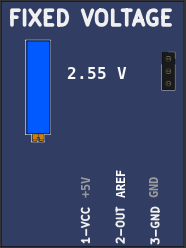
\includegraphics[width=0.3\textwidth]{img/part_fixedv.png} 
\end{figure} 


\href{https://lcgamboa.github.io/picsimlab_examples/parts_Fixed_Voltage.html}{Examples}

 
\subsection{Gamepad}

This part is a gamepad with two analog axis and 7 push buttons.

\begin{figure}[H]
\center
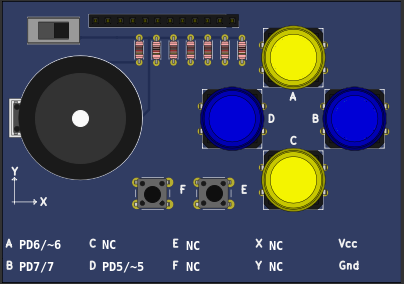
\includegraphics[width=0.6\textwidth]{img/part_gamepad.png} 
\end{figure} 

\begin{figure}[H]
\center
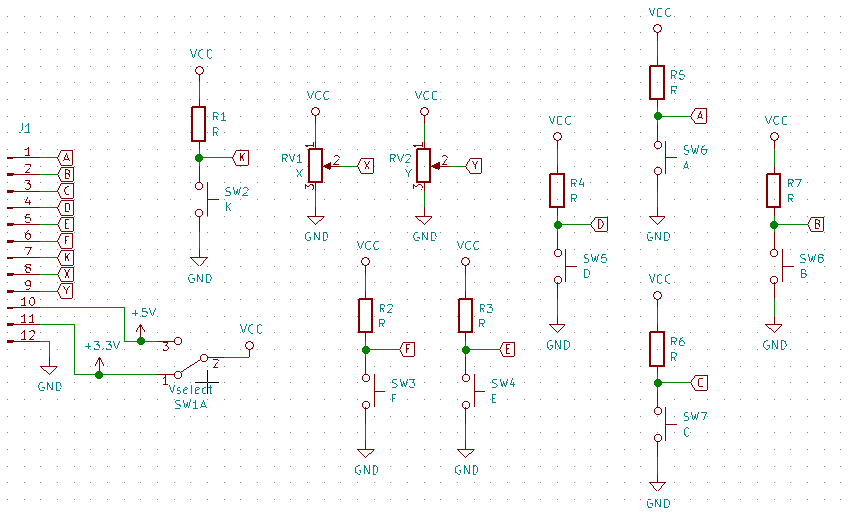
\includegraphics[width=0.99\textwidth]{img/part_gamepad_.png} 
\end{figure} 

The gamepad can be controlled by keyboards keys:
\begin{itemize}
 \item X axis - keys 'A' and 'D'
 \item Y axis - keys 'W' and 'S'
 \item Button A - key 'I'
 \item Button B - key 'L'
 \item Button C - key 'K'
 \item Button D - key 'J'
 \item Button E - key 'E'
 \item Button F - key 'O'
 \item Button K - key 'R'
\end{itemize}


\href{https://lcgamboa.github.io/picsimlab_examples/parts_Gamepad.html}{Examples}

\subsection{Gamepad (Analogic)}

This part is a gamepad with 5 push buttons and one analogic output.

\begin{figure}[H]
\center
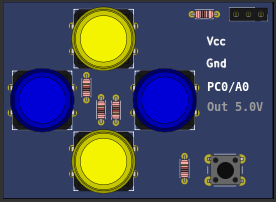
\includegraphics[width=0.4\textwidth]{img/part_gamepad_an.png} 
\end{figure} 


The gamepad can be controlled by keyboards keys:
\begin{itemize}
 \item Button A - key 'L'
 \item Button B - key 'I'
 \item Button C - key 'K'
 \item Button D - key 'J'
 \item Button E - key 'O'
 \end{itemize}


\href{https://lcgamboa.github.io/picsimlab_examples/parts_Gamepad_(Analogic).html}{Examples}

\subsection{Keypad}

It is a matrix keyboard configurable to 4x3 , 4x4 or 2x5 rows/columns.

\begin{figure}[H]
\center
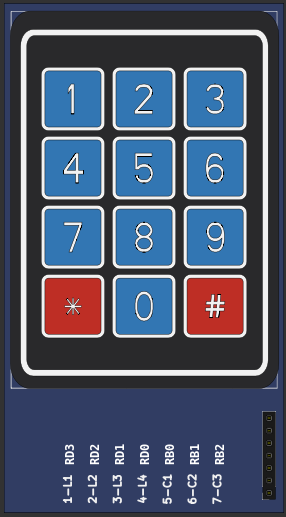
\includegraphics[width=0.33\textwidth]{img/part_keyb_4x3.png} 
\end{figure} 

\begin{figure}[H]
\center
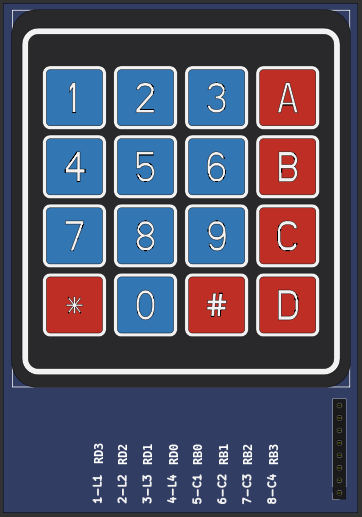
\includegraphics[width=0.4\textwidth]{img/part_keyb_4x4.png} 
\end{figure} 

\begin{figure}[H]
\center
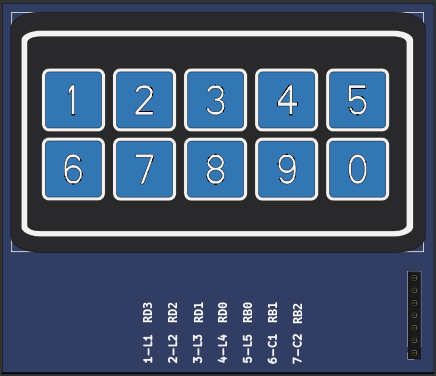
\includegraphics[width=0.5\textwidth]{img/part_keyb_2x5.png} 
\end{figure} 

\href{https://lcgamboa.github.io/picsimlab_examples/parts_Keypad.html}{Examples}


\subsection{LDR}

This part is light dependent resistor (LDR) connected in series with one 10K resistor.
The analog output of the voltage divider is applied to one voltage follower and can be 
read directly from pin A0.
The analog value from voltage follower is compared with one voltage threshold, the digital 
output of comparator and can be read directly from pin D0.

\begin{center}
\begin{tabular}{l|c}
\hline LDR Characteristics  & Value \\
\hline 
\hline Gamma value at 100-10Lux       &       0.7\\
\hline Light Resistance at 10Lux (25°C) &     20K$\Omega$\\
\hline 
\end{tabular}
\end{center}


\begin{figure}[H]
\center
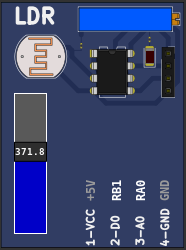
\includegraphics[width=0.3\textwidth]{img/part_LDR.png} 
\end{figure} 

\begin{figure}[H]
\center
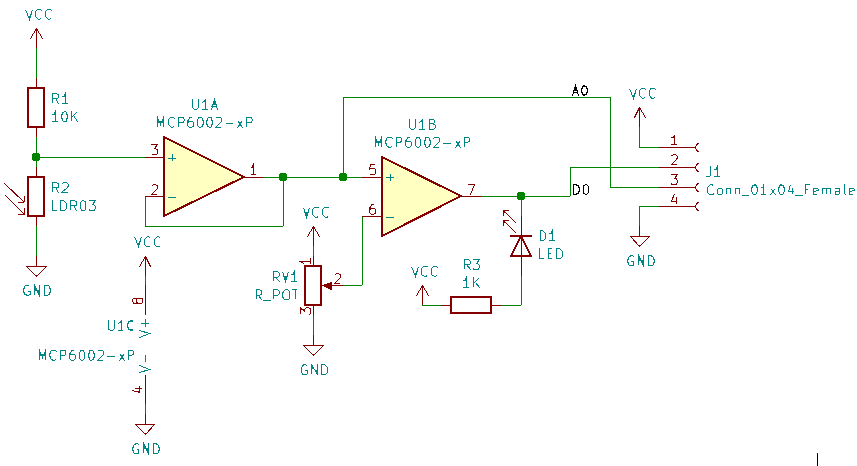
\includegraphics[width=0.8\textwidth]{img/part_LDR_.png} 
\end{figure} 


\href{https://lcgamboa.github.io/picsimlab_examples/parts_LDR.html}{Examples}


\subsection{LM35 (Temperature)}

This part is LM35 analog temperature sensor. The measurement range is 2 to 150 °C  and 
voltage output is 10mV/°C.

\begin{figure}[H]
\center
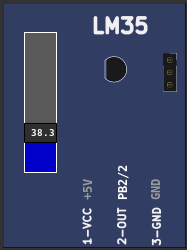
\includegraphics[width=0.3\textwidth]{img/part_lm35.png} 
\end{figure} 


\href{https://lcgamboa.github.io/picsimlab_examples/parts_LM35_(Temperature).html}{Examples}


\subsection{MPU6050}

This part is MPU6050 accelerometer and gyroscope with I2C interface. 
Only raw values are available, DMP is not supported.

\begin{figure}[H]
\center
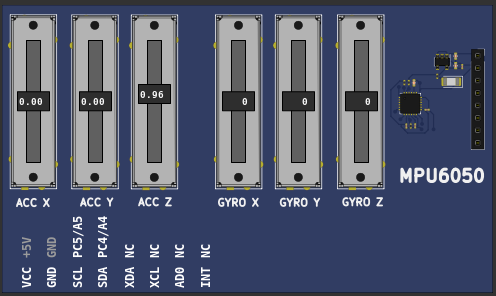
\includegraphics[width=0.6\textwidth]{img/part_mpu6050.png} 
\end{figure} 


\href{https://lcgamboa.github.io/picsimlab_examples/parts_MPU6050.html}{Examples}

\subsection{Potentiometers}

This part is formed by 4 potentiometers connected between 0 and 5 volts, the output is connected to the cursor and varies within this voltage range.
\begin{figure}[H]
\center
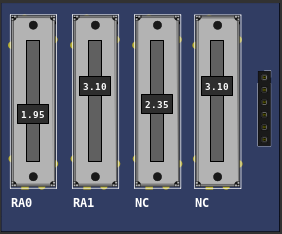
\includegraphics[width=0.6\textwidth]{img/part_pot.png} 
\end{figure} 

\begin{figure}[H]
\center
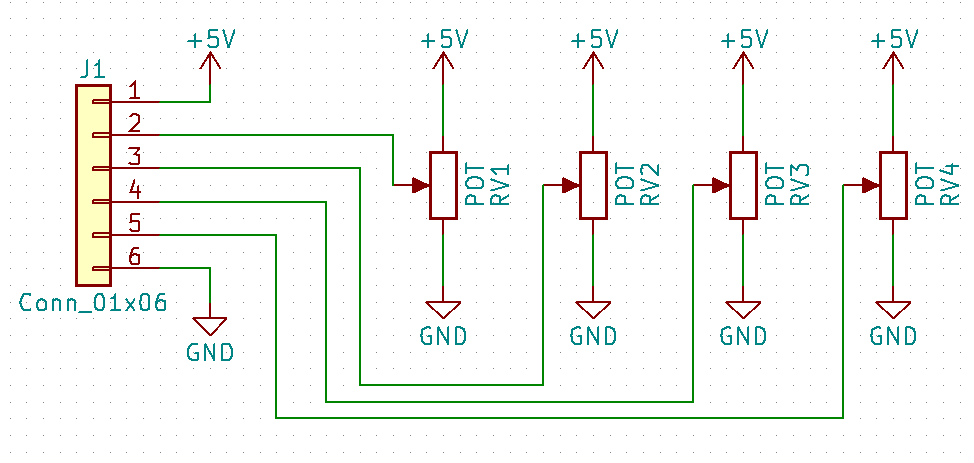
\includegraphics[width=0.8\textwidth]{img/part_pot_.png} 
\end{figure} 

\href{https://lcgamboa.github.io/picsimlab_examples/parts_Potentiometers.html}{Examples}

\subsection{Potentiometers (Rotary)}

This part is formed by 4 rotary potentiometers connected between 0 and 5 volts, the output is connected to the cursor and varies within this voltage range.
\begin{figure}[H]
\center
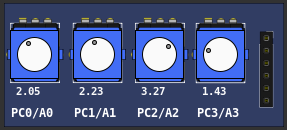
\includegraphics[width=0.6\textwidth]{img/part_pot_r.png} 
\end{figure} 

\begin{figure}[H]
\center
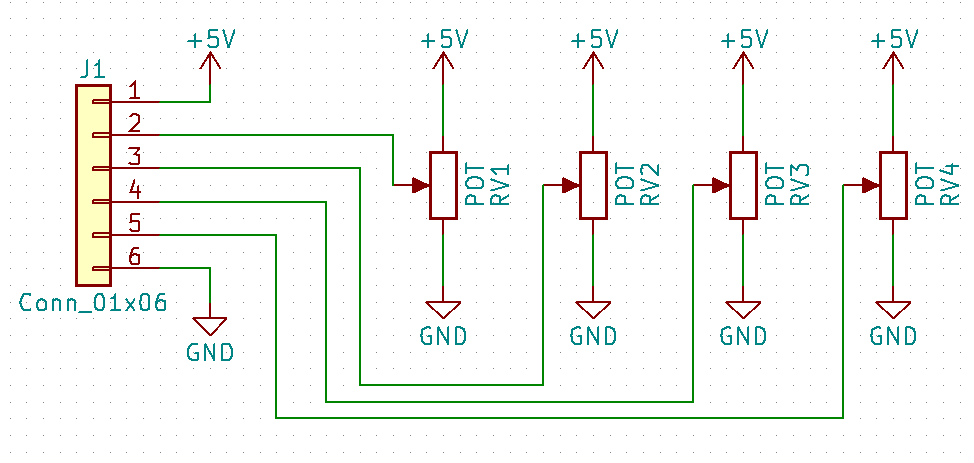
\includegraphics[width=0.8\textwidth]{img/part_pot_.png} 
\end{figure} 

\href{https://lcgamboa.github.io/picsimlab_examples/parts_Potentiometers_(Rotary).html}{Examples}

\subsection{Push Buttons}

This part consists of 8 push buttons. The output active state can be configurable.
The buttons have activation bounce effect emulation. 
\begin{figure}[H]
\center
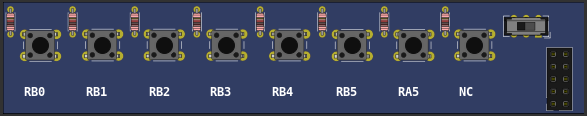
\includegraphics[width=0.99\textwidth]{img/part_buttons.png} 
\end{figure} 

\begin{figure}[H]
\center
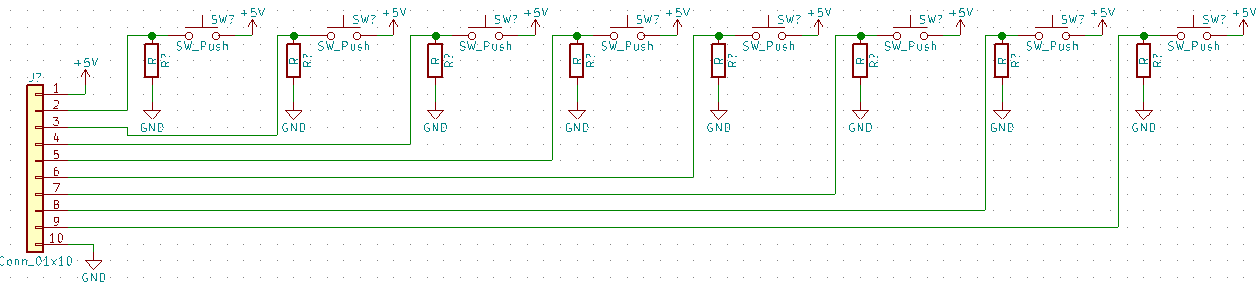
\includegraphics[width=0.99\textwidth]{img/part_buttons_.png} 
\end{figure} 

\href{https://lcgamboa.github.io/picsimlab_examples/parts_Push_Buttons.html}{Examples}


\subsection{Push Buttons (Analogic)}


This part consists of 8 push buttons connected in a resistive ladder.

\begin{figure}[H]
\center
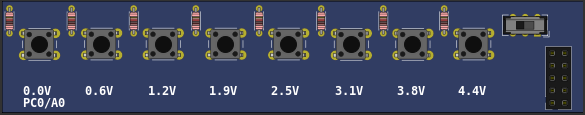
\includegraphics[width=0.99\textwidth]{img/part_push_a.png} 
\end{figure}

\href{https://lcgamboa.github.io/picsimlab_examples/parts_Push_Buttons_(Analogic).html}{Examples}

\subsection{SHT3X (Temp. Hum.)}

This part is SHT3X analog temperature and humidity sensor. The temperature  range is -40 to 125 °C  and 
voltage output is 22.85mV/°C + 1.53V . The relative humidity range is 0 to 100 \%  and voltage output is 40mV/\% + 500mV.

\begin{figure}[H]
\center
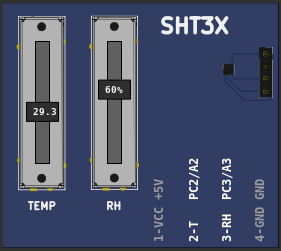
\includegraphics[width=0.5\textwidth]{img/part_sht3x.png} 
\end{figure} 


\href{https://lcgamboa.github.io/picsimlab_examples/parts_SHT3X_(Temp._Hum.).html}{Examples}



\subsection{Switches}
This part consists of 8 switches with on or off position (0 or 1).
The switches have activation bounce effect emulation.

\begin{figure}[H]
\center
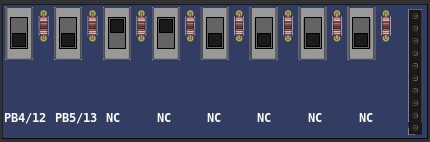
\includegraphics[width=0.99\textwidth]{img/part_switches.png} 
\end{figure} 

\begin{figure}[H]
\center
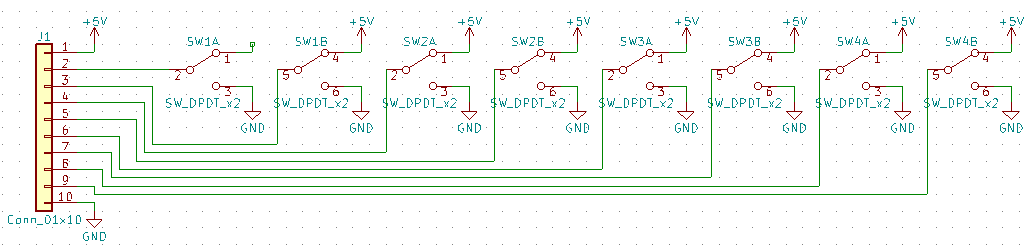
\includegraphics[width=0.99\textwidth]{img/part_switches_.png} 
\end{figure} 

\href{https://lcgamboa.github.io/picsimlab_examples/parts_Switches.html}{Examples}



\subsection{Ultrasonic HC-SR04}
This part is ultrasonic range meter sensor.

\begin{figure}[H]
\center
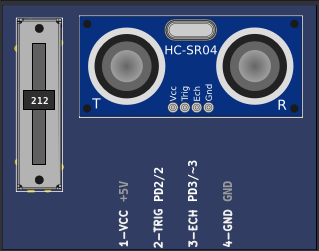
\includegraphics[width=0.4\textwidth]{img/part_hcsr04.png} 
\end{figure} 


\href{https://lcgamboa.github.io/picsimlab_examples/parts_Ultrasonic_HC-SR04.html}{Examples}



\section{Outputs}

\subsection{7 Segments Display}

This part can be configured as four multiplexed or one single 7 segments display.

\subsubsection{Four Multiplexed}
\begin{figure}[H]
\center
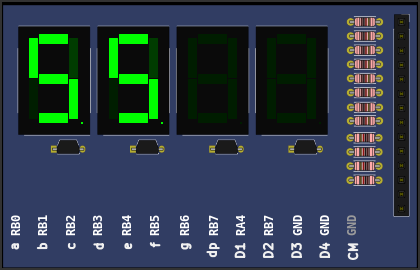
\includegraphics[width=0.5\textwidth]{img/part_7seg.png} 
\end{figure} 

\begin{figure}[H]
\center
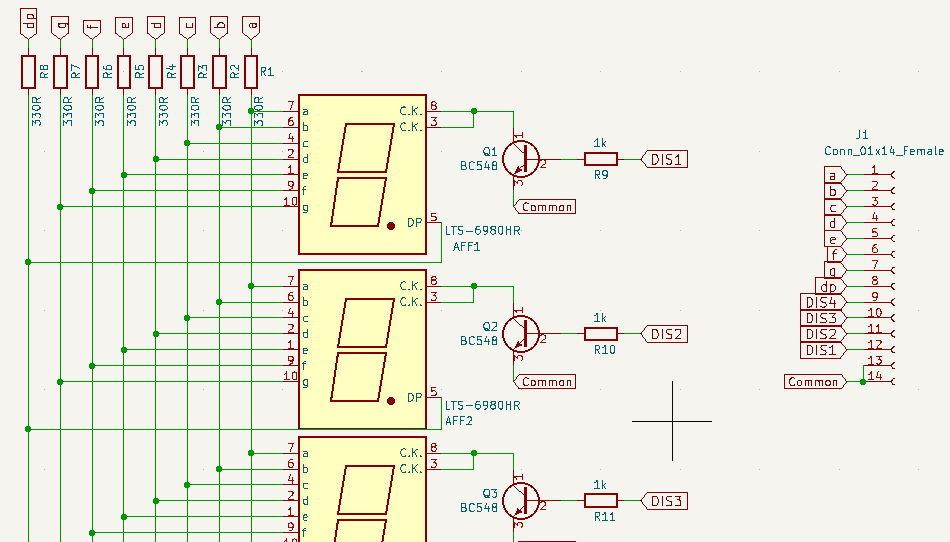
\includegraphics[width=0.9\textwidth]{img/part_7seg_.png} 
\end{figure} 


\subsubsection{Single Display}
\begin{figure}[H]
\center
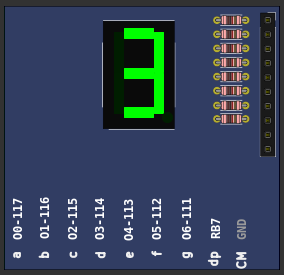
\includegraphics[width=0.35\textwidth]{img/part_7seg1.png} 
\end{figure} 

\begin{figure}[H]
\center
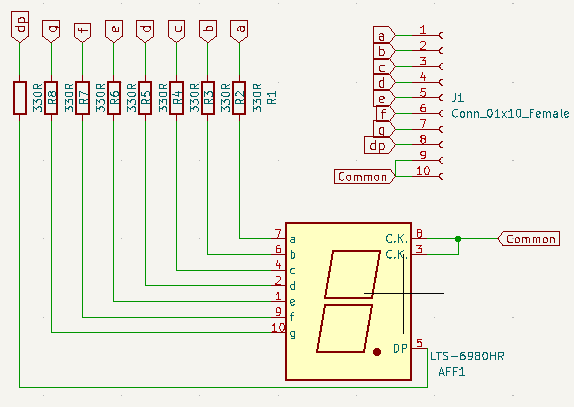
\includegraphics[width=0.7\textwidth]{img/part_7seg1_.png} 
\end{figure} 


\href{https://lcgamboa.github.io/picsimlab_examples/parts_7_Segments_Display.html}{Examples}

\subsection{7 Segments Display (Decoder)}

This is a four multiplexed 7 segments displays with BCD to 7 segments decoder (CD4511).


\subsubsection{Four Multiplexed}
\begin{figure}[H]
\center
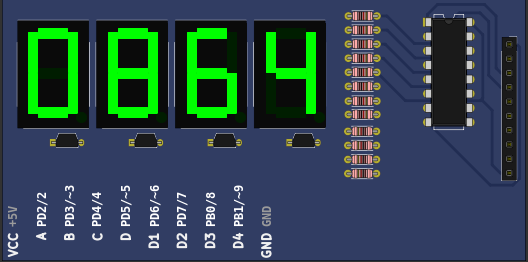
\includegraphics[width=0.6\textwidth]{img/part_7seg_dec.png} 
\end{figure} 

\begin{figure}[H]
\center
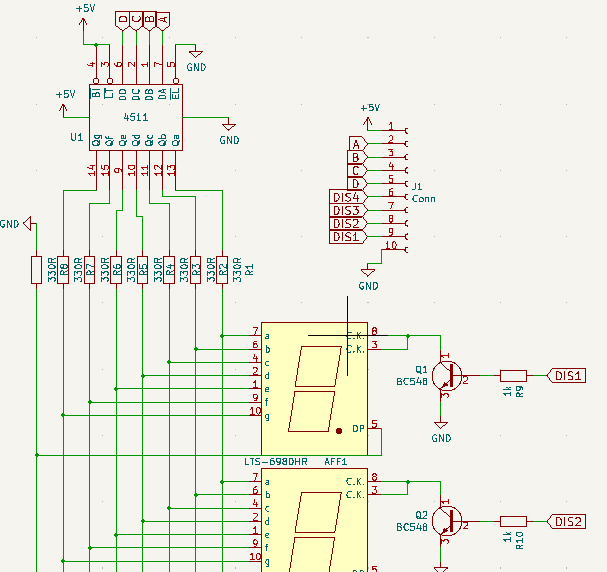
\includegraphics[width=0.8\textwidth]{img/part_7seg_dec_.png} 
\end{figure} 

\subsubsection{Four with Latch}
\begin{figure}[H]
\center
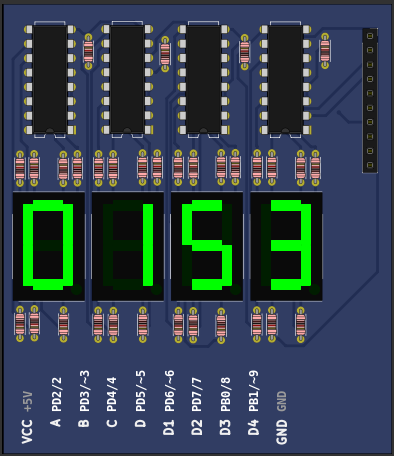
\includegraphics[width=0.5\textwidth]{img/part_7seg_latch.png} 
\end{figure} 


\begin{figure}[H]
\center
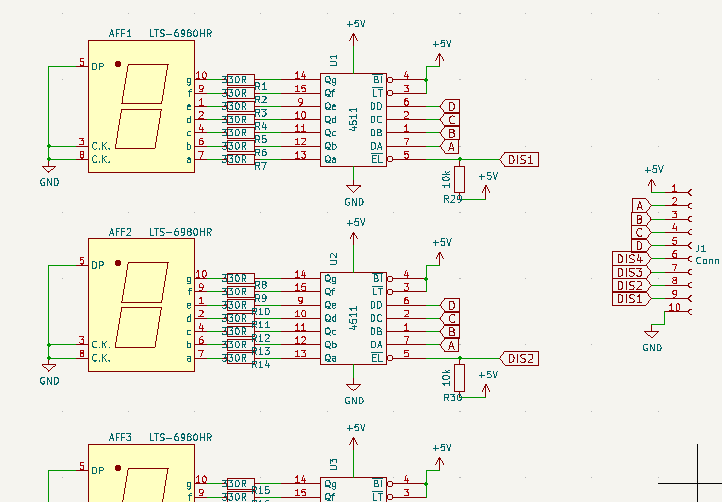
\includegraphics[width=0.9\textwidth]{img/part_7seg_latch_.png} 
\end{figure} 

\href{https://lcgamboa.github.io/picsimlab_examples/parts_7_Segments_Display_(Decoder).html}{Examples}

\subsection{Buzzer}

This is a active/passive buzzer.
The buzzer has 3 operating modes: 
\begin{itemize}
\item \textbf{Active}: When powered, the buzzer emits a frequency of 440Hz. 
\item \textbf{Passive}: In this mode the values read from the input pin are sent directly to the sound card, this mode only works well if the simulation is in real time. 
\item \textbf{Tone}: This second passive mode measures the frequency on the input and updates the frequency of the buzzer every 100ms, its accuracy is less than the normal passive mode but it works better when the simulation is not in real time. 
\end{itemize}

\begin{figure}[H]
\center
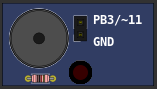
\includegraphics[width=0.2\textwidth]{img/part_buzzer.png} 
\end{figure} 

\href{https://lcgamboa.github.io/picsimlab_examples/parts_Buzzer.html}{Examples}


\subsection{DC Motor}

This part is DC motor with H-bridge driver and quadrature encoder. 

\begin{figure}[H]
\center
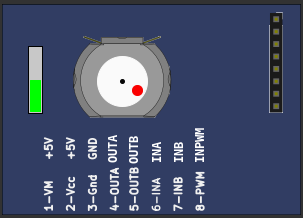
\includegraphics[width=0.4\textwidth]{img/part_dcmotor.png} 
\end{figure} 

\begin{figure}[H]
\center
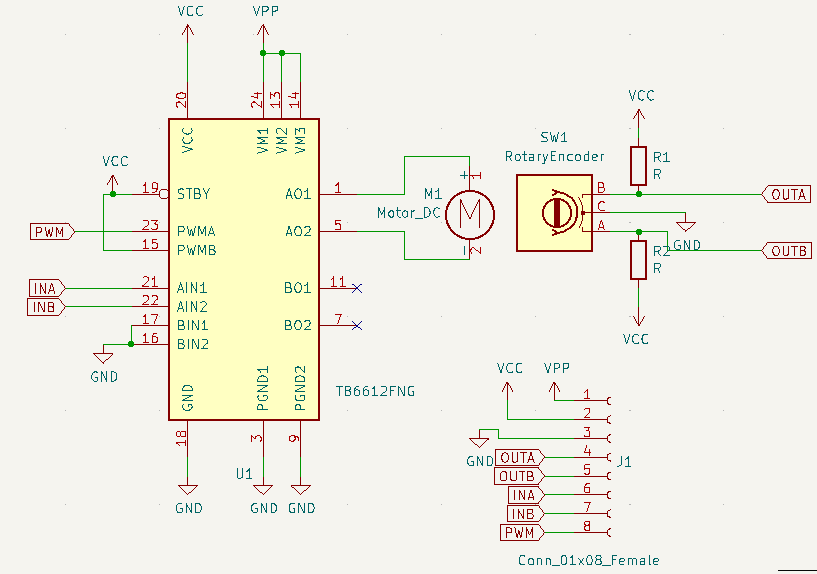
\includegraphics[width=0.8\textwidth]{img/part_dcmotor_.png} 
\end{figure} 

\href{https://lcgamboa.github.io/picsimlab_examples/parts_DC_Motor.html}{Examples}


\subsection{LCD hd44780}

This part is a text display with 2 (or 4) lines by 16 (or 20) columns.

\begin{figure}[H]
\center
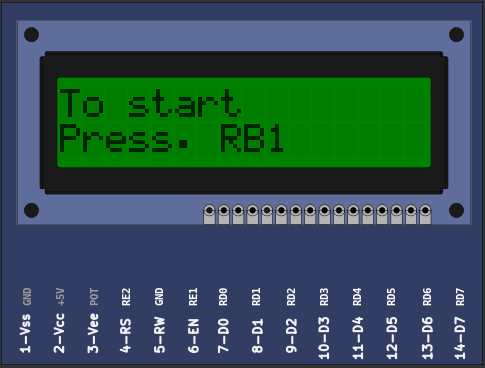
\includegraphics[width=0.6\textwidth]{img/part_hd44780_2x16.png} 
\end{figure} 

\begin{figure}[H]
\center
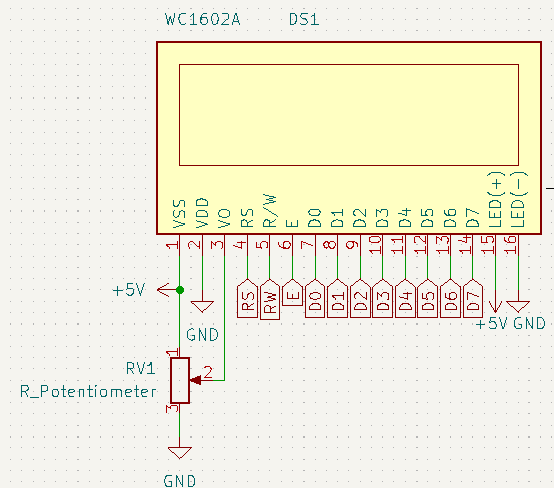
\includegraphics[width=0.6\textwidth]{img/part_hd44780_2x16_.png} 
\end{figure} 


\begin{figure}[H]
\center
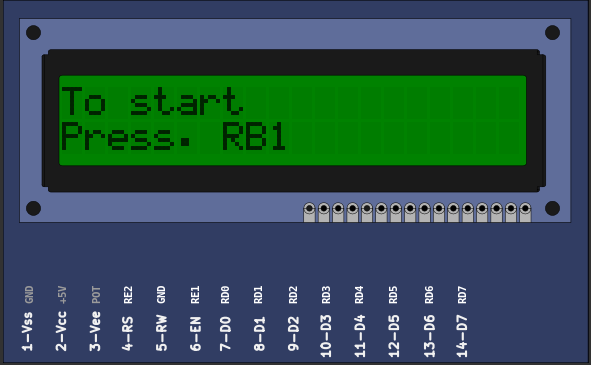
\includegraphics[width=0.7\textwidth]{img/part_hd44780_2x20.png} 
\end{figure} 

\begin{figure}[H]
\center
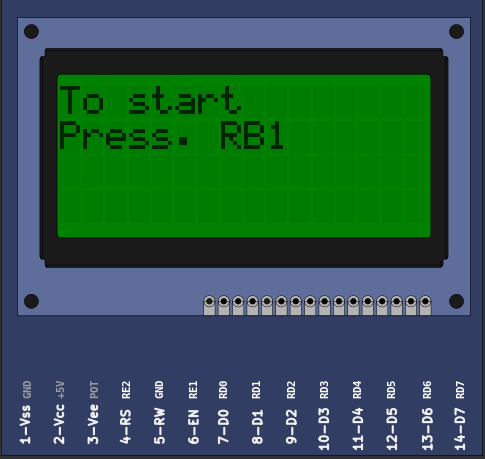
\includegraphics[width=0.6\textwidth]{img/part_hd44780_4x16.png} 
\end{figure} 

\begin{figure}[H]
\center
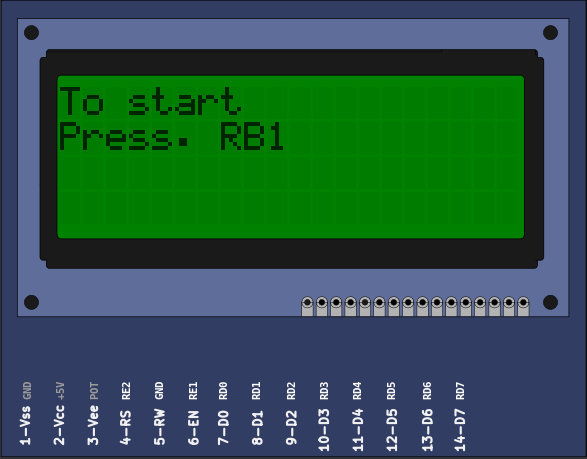
\includegraphics[width=0.7\textwidth]{img/part_hd44780_4x20.png} 
\end{figure} 

\href{https://lcgamboa.github.io/picsimlab_examples/parts_LCD_hd44780.html}{Examples}

\subsection{LCD ili9341}

This part is a color graphic display with 240x320 pixels with touchscreen (xpt2046 controller).
Only 4 SPI mode and 8 bits parallel mode is avaliable.

\begin{figure}[H]
\center
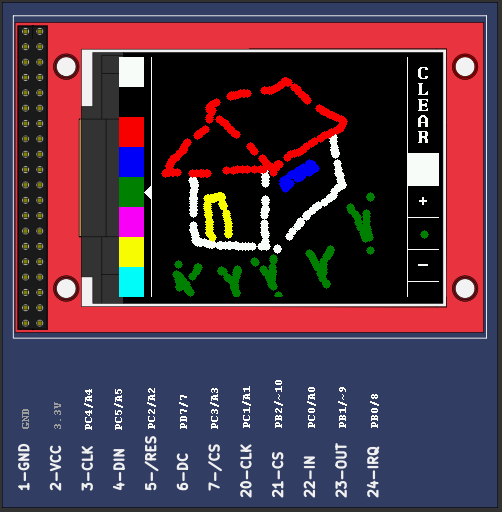
\includegraphics[width=0.7\textwidth]{img/part_lcd_ili9341.png} 
\end{figure} 

\href{https://lcgamboa.github.io/picsimlab_examples/parts_LCD_ili9341.html}{Examples}


\subsection{LCD pcf8833}

This part is a color graphic display with 132x132 pixels.

\begin{figure}[H]
\center
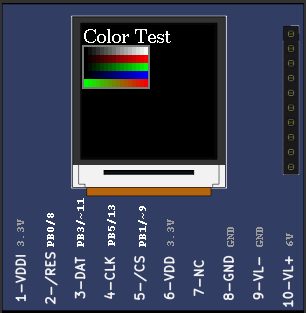
\includegraphics[width=0.4\textwidth]{img/part_pcf8833.png} 
\end{figure} 

\href{https://lcgamboa.github.io/picsimlab_examples/parts_LCD_pcf8833.html}{Examples}


\subsection{LCD pcd8544 }

This part is a monochrome graphic display with 48x84 pixels. (Nokia 5110)

\begin{figure}[H]
\center
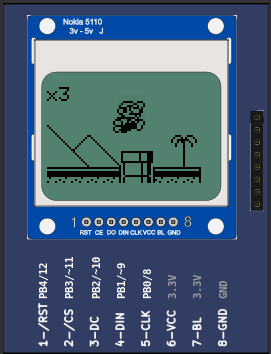
\includegraphics[width=0.35\textwidth]{img/part_pcd8544.png} 
\end{figure} 

\href{https://lcgamboa.github.io/picsimlab_examples/parts_LCD_pcd8544.html}{Examples}

\subsection{LCD ssd1306 }

This part is a monochrome oled graphic display with 128x64 pixels. 
The part suport I2C and 4 SPI serial mode.

\begin{figure}[H]
\center
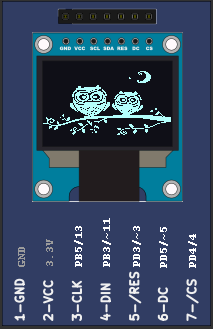
\includegraphics[width=0.35\textwidth]{img/part_lcd_ssd1306.png} 
\end{figure} 

\href{https://lcgamboa.github.io/picsimlab_examples/parts_LCD_ssd1306.html}{Examples}


\subsection{LED Matrix}

It is a 8x8 LED matrix with MAX72xx controller.

\begin{figure}[H]
\center
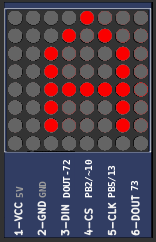
\includegraphics[width=0.4\textwidth]{img/part_LED_matrix.png} 
\end{figure}

\href{https://lcgamboa.github.io/picsimlab_examples/parts_LED_Matrix.html}{Examples}

\subsection{LEDs}

This part is a bar of 8 independent colored LEDs.

\begin{figure}[H]
\center
\includegraphics[width=0.99\textwidth]{img/part_leds.png} 
\end{figure} 

\begin{figure}[H]
\center
\includegraphics[width=0.8\textwidth]{img/part_leds_.png} 
\end{figure} 

\href{https://lcgamboa.github.io/picsimlab_examples/parts_LEDs.html}{Examples}
 
\subsection{RGB LED}

This part consists of a 4-pin RGB LED. Each color can be triggered independently.
Using PWM it is possible to generate several colors by combining the 3 primary colors. 
\begin{figure}[H]
\center
\includegraphics[width=0.4\textwidth]{img/part_rgb.png} 
\end{figure} 

\begin{figure}[H]
\center
\includegraphics[width=0.6\textwidth]{img/part_rgb_.png} 
\end{figure} 

\href{https://lcgamboa.github.io/picsimlab_examples/parts_RGB_LED.html}{Examples}


\subsection{RGB LED WS2812B}

This part consists of a addressable RGB LED WS2812B. It is possible to set the number 
of rows and columns in the configuration window. The LED can be used with or without diffuser. 

\begin{figure}[H]
\center
\includegraphics[width=0.9\textwidth]{img/part_led_ws2812b.png} 
\end{figure} 


\href{https://lcgamboa.github.io/picsimlab_examples/parts_RGB_LED_WS2812B.html}{Examples}

\subsection{Servo Motor}

The servo motor is a component that must be activated with a pulse of variable width from 1ms to 2ms every 20 ms.
A pulse of 1ms positions the servo at -90º, one from 1.5ms to 0º and one from 2ms to 90º.

\begin{figure}[H]
\center
\includegraphics[width=0.4\textwidth]{img/part_servo.png} 
\end{figure} 

\begin{figure}[H]
\center
\includegraphics[width=0.8\textwidth]{img/part_servo_.png} 
\end{figure} 

\href{https://lcgamboa.github.io/picsimlab_examples/parts_Servo_Motor.html}{Examples}


\subsection{Step Motor}

The stepper motor is a component with 4 coils that must be driven in the correct order to rotate the rotor.
Each step of the motor is 1.8º.

\begin{figure}[H]
\center
\includegraphics[width=0.5\textwidth]{img/part_step.png} 
\end{figure} 

\begin{figure}[H]
\center
\includegraphics[width=0.99\textwidth]{img/part_step_.png} 
\end{figure} 

\href{https://lcgamboa.github.io/picsimlab_examples/parts_Step_Motor.html}{Examples}



\section{Others}


\subsection{ETH w5500}

This part is a ethernet shield w5500 with support to 8 sockets simultaneously.

Only TCP/UDP unicast address sockets is supported. 
DHCP is emulated and return a fake ipv4 address.

All listening ports below 2000 are increased by 2000 to avoid operational system services ports. 
For example listening on port 80 becomes 2080. 

w5500 Status Legend:
\begin{center}
\begin{tabular}{l|l|l}
\hline \textbf{1º Letter - Type} & \textbf{2º Letter - Status} & \textbf{3º Letter - Error}\\
\hline
\hline C - Closed & C - Closed & B - Bind\\
\hline T - TCP & I - Initialized & S - Send\\
\hline U - UDP & L - Listen & R - Receive\\
\hline M - MACRAW (don't supported) & S - Syn sent & L - Listen\\
\hline   & E - Established & U - Reuse\\
\hline   & W - Close wait & C - Connecting\\
\hline   & U - UDP & D - Shutdown\\
\hline   & M - MACRAW (don't supported) &   \\
\hline
\end{tabular}
\end{center}

Click on connector to toggle link status.

\begin{figure}[H]
\center
\includegraphics[width=0.6\textwidth]{img/part_w5500.png} 
\end{figure} 

\href{https://lcgamboa.github.io/picsimlab_examples/parts_ETH_w5500.html}{Examples}
 

\subsection{IO 74xx573}

This is one 74xx573 octal latch.

\begin{figure}[H]
\center
\includegraphics[width=0.35\textwidth]{img/part_74xx573.png} 
\end{figure} 

\href{https://lcgamboa.github.io/picsimlab_examples/parts_IO_74xx573.html}{Examples} 

\subsection{IO 74xx595}

This is one 74xx595 serial input and parallel output 8 bit shift register.

\begin{figure}[H]
\center
\includegraphics[width=0.6\textwidth]{img/part_74xx595.png} 
\end{figure} 

\href{https://lcgamboa.github.io/picsimlab_examples/parts_IO_74xx595.html}{Examples}

\subsection{IO MCP23S17}

It is a MCP23S17 serial SPI IO expander part.

\begin{figure}[H]
\center
\includegraphics[width=0.6\textwidth]{img/part_MCP23S17.png} 
\end{figure} 

\href{https://lcgamboa.github.io/picsimlab_examples/parts_IO_MCP23S17.html}{Examples}

\subsection{IO PCF8574}

It is a PCF8574 serial I2C IO expander.

\begin{figure}[H]
\center
\includegraphics[width=0.6\textwidth]{img/part_pcf8574.png} 
\end{figure} 

\href{https://lcgamboa.github.io/picsimlab_examples/parts_IO_PCF8574.html}{Examples}


\subsection{IO UART}

This part is a UART serial port. This part connects the hardware/software UART IO pins of microcontroller to
one real/virtual PC serial port. To use virtual port is need to install a virtual port software, as 
described in Chapter: \hyperlink{def:seriali}{Serial Communication}. 
The serial communication uses the 8N1 format.

\begin{figure}[H]
\center
\includegraphics[width=0.6\textwidth]{img/part_uart.png} 
\end{figure} 

\href{https://lcgamboa.github.io/picsimlab_examples/parts_IO_UART.html}{Examples}


\subsection{Jumper Wires}

This part are formed by sixteen jumper wires. Each jumper has one input and one output.  The jumper input must be connected to one pin output, 
the jumper output can be connected to multiple pin inputs. The jumper can be used to connect microcontroller pins or make connection between 
spare parts pins.   

\begin{figure}[H]
\center
\includegraphics[width=0.6\textwidth]{img/part_jumper.png} 
\end{figure} 

\href{https://lcgamboa.github.io/picsimlab_examples/parts_Jumper_Wires.html}{Examples}

\subsection{MEM 24CXXX}

It is a 24CXXX serial I2C EEPROM part. There are support to the models 24C04 and 24C512.

\begin{figure}[H]
\center
\includegraphics[width=0.4\textwidth]{img/part_mem24xx.png} 
\end{figure}

\href{https://lcgamboa.github.io/picsimlab_examples/parts_MEM_24CXXX.html}{Examples}

\subsection{RTC ds1307}

This part is a ds1307 real time clock with serial I2C interface.

\begin{figure}[H]
\center
\includegraphics[width=0.4\textwidth]{img/part_ds1307.png} 
\end{figure}

\href{https://lcgamboa.github.io/picsimlab_examples/parts_RTC_ds1307.html}{Examples}


\subsection{RTC pfc8563}

This part is a pfc8563 real time clock with serial I2C interface.

\begin{figure}[H]
\center
\includegraphics[width=0.4\textwidth]{img/part_pcf8563.png} 
\end{figure}

\href{https://lcgamboa.github.io/picsimlab_examples/parts_RTC_pfc8563.html}{Examples}


\subsection{SD Card}

This part is a SD Card shield. It's necessary set one sd card file image before use it. (Click on SD card connector to open file dialog)

On Linux one empty image can be created with this command: 
\begin{verbatim}
 dd if=/dev/zero of=sd.img bs=1M count=32
\end{verbatim}
This empty image can be used with raw SD card access, to work with FAT file system  the image need to be formatted before the use. (using \href{https://github.com/greiman/SdFat/blob/master/examples/SdFormatter/SdFormatter.ino}{SdFormatter.ino} for example) 

\begin{figure}[H]
\center
\includegraphics[width=0.6\textwidth]{img/part_sdcard.png} 
\end{figure} 

\begin{figure}[H]
\center
\includegraphics[width=0.8\textwidth]{img/part_sdcard_.png} 
\end{figure} 


\href{https://lcgamboa.github.io/picsimlab_examples/parts_SD_Card.html}{Examples}


\subsection{Temperature System}

This part is a temperature control system. 
The temperature control system consists of a heating resistor, an LM35 temperature sensor, 
a cooler and an infrared tachometer.


\begin{figure}[H]
\center
\includegraphics[width=0.65\textwidth]{img/part_tempsys.png} 
\end{figure}

\href{https://lcgamboa.github.io/picsimlab_examples/parts_Temperature_System.html}{Examples}

\section{Virtual}

\subsection{D. Transfer Function}

This is a discrete transfer function mathematical model. 

\begin{figure}[H]
\center
\includegraphics[width=0.9\textwidth]{img/part_dtransferf.png} 
\end{figure} 

\href{https://lcgamboa.github.io/picsimlab_examples/parts_D._Transfer_Function.html}{Examples}

\subsection{IO Virtual Term} \hypertarget{def:vterm}{}

This part is a virtual serial terminal. This part can be used to read and write RX/TX pins UART signals.
To use this part are don't need to use or install one virtual serial ports on computer.  
Clik on terminal picture to open the terminal window.
The serial communication uses the 8N1 format.

\begin{figure}[H]
\center
\includegraphics[width=0.99\textwidth]{img/part_vterm.png} 
\end{figure} 

\href{https://lcgamboa.github.io/picsimlab_examples/parts_IO_Virtual_Term.html}{Examples}

\subsection{Signal Generator}

This part is a virtual signal generator with support for sine, square and triangular waves 
generation with amplitude and frequency adjustment.

\begin{figure}[H]
\center
\includegraphics[width=0.4\textwidth]{img/part_sgen.png} 
\end{figure}

\href{https://lcgamboa.github.io/picsimlab_examples/parts_Signal_Generator.html}{Examples}


\subsection{Text Box}

This part is static multiline text box. 

\begin{figure}[H]
\center
\includegraphics[width=0.7\textwidth]{img/part_text_box.png} 
\end{figure}


\href{https://lcgamboa.github.io/picsimlab_examples/parts_Text_Box.html}{Examples}


\subsection{VCD Dump}

This part is a digital value file dump (VCD) recorder. The VCD generated file can be visualized with one external viewer like 
\hrefb{https://sourceforge.net/projects/gtkwave/files/}{gtkwave} or \hrefb{https://sigrok.org/wiki/Downloads}{pulseview}. 

\begin{figure}[H]
\center
\includegraphics[width=0.8\textwidth]{img/part_vcd_dump.png} 
\end{figure}



\begin{figure}[H]
\center
\includegraphics[width=0.99\textwidth]{img/part_vcd_dump_gtkwave.png} 
\end{figure}

\href{https://lcgamboa.github.io/picsimlab_examples/parts_VCD_Dump.html}{Examples}


\subsection{VCD Dump (Analogic)}


This part is a analog value file dump (VCD) recorder. The VCD generated file can be visualized with one external viewer like 
\hrefb{https://sourceforge.net/projects/gtkwave/files/}{gtkwave} or \hrefb{https://sigrok.org/wiki/Downloads}{pulseview}.  

\begin{figure}[H]
\center
\includegraphics[width=0.8\textwidth]{img/part_vcd_dump_an.png} 
\end{figure}



\begin{figure}[H]
\center
\includegraphics[width=0.99\textwidth]{img/part_vcd_dump_gtkwave_an.png} 
\end{figure}

\href{https://lcgamboa.github.io/picsimlab_examples/parts_VCD_Dump_(Analogic).html}{Examples}

 
\subsection{VCD Play}


This part play a VCD file generated from VCD Dump part.  

\begin{figure}[H]
\center
\includegraphics[width=0.8\textwidth]{img/part_vcd_play.png} 
\end{figure}


\href{https://lcgamboa.github.io/picsimlab_examples/parts_VCD_Play.html}{Examples}

